\documentclass{article}
\usepackage{amsmath,amsthm,amssymb}
\usepackage{mathtext}
\usepackage[T2A]{fontenc}
\usepackage[utf8]{inputenc}
\usepackage[english]{babel}
\usepackage{graphicx}
\usepackage{hyperref}
\usepackage{indentfirst}
\usepackage{float}

\title{Yet Another Conditional Headline Generation (Yachg)}
\author{Valetov D.K., Butov R.A.}
\date{May 2020}



\begin{document}
\maketitle
\begin{abstract}
	Large-scale  language  models  show  promising  results in text  generation  tasks. Several methods on conditional generation exists.  We release another one, based on classic transformer with aim to enable text generating control via adding to source sequence an aspect vector produced by unsupervised aspect model.
	Code can be assessed in repository: \url{https://github.com/DmitriyValetov/nlp_course_project}.
\end{abstract}
\section{Introduction}
More the people, more texts they write, more time is spent in mining texts on related works, news, articles, less time for the nearest and dearest. Time spent on text surfing can be significantly reduced by good means of summarization, which will allow us not to dive into materials that do not correspond to our interests. Summarization is an important challenge of natural language understanding. The aim is to produce a  shorten  representation  of  an  input  text  that captures the main meaning ideas of the original text. Aim of this paper is to hybridize topic modelling and summarization. Particularly - to use aspects vectors in the summary generation process and check whether an aspect can influence the result of summing text  E.g. generate a different summary of the text by bias to one or more of its topics.

\subsection{Team}

\textbf{Valetov Dmitriy}: Data processing, implementing ABAE, conditioning a transformer with ABAE aspect vector.

\textbf{Butov Roman}: Data processing, metrics assessing, inference methods.

\section{Related Work}
Base of our problem is classic sequence-to-sequence problem, we need an instrument to generate target sequence with known source sequence. There are two main types of summarization - extractive and abstractive. First extracts some key words from source sequence, and the second generates a fresh text extracting some latent information. Our problem is of the second type. 

There are numerous works about text summation with recurrent neural networks \cite{nallapati2016abstractive, li2017deep} and with transformers: \cite{zhang2019hibert, hoang2019efficient}. 

Works on conditional text generation similar to described in this paper could be found here: \cite{keskar2019ctrl, xia2020cg}. The CTRL model is a language model that was trained to generate text with embedded tokens for conditioning the process like: "Horror lore", "Wikipedia article", "Books" etc.

\section{Model Description}
Base of our model is a classic transformer \cite{vaswani2017attention}. We used a classical implementation of transformer from Pytorch. 

To make generation conditional we use sentiment extraction model (ABAE) from \cite{he2017unsupervised} to get most relative aspect vector for a given source sequence of tokens. Then we prepend this aspect vector to the given embedded source sequence (like it is done in \cite{keskar2019ctrl}) and feed it in transformer. That's nearly all the model. 

\section{Dataset}
Rossiya Segodnya dataset has been used \cite{RiaRepoUrl}.
We did several text normalizations: lemmatization with stopwords, BPE and raw text.
First of all we did html parcing with BeautifulSoup package \cite{richardson2007beautiful}. Sentence and word tokenization made by NLTK \cite{Loper02nltk:the} package. For lemmatiztion we used pymorphy2 package \cite{pymorphy2}. Stopwords list obtained from NLTK package. For BPE we used youtokentome package \cite{youtokentome}. 

\begin{table}[H]
\begin{center}
\begin{tabular}[t]{|l|cccc|}
\hline
%\cline{2-4}
Type &  unique tokens & total tokens & vocabulary & tokens in vocabulary \\
\hline
lem+stop & 600k & 200M & 50k & 196M (~98\%) \\
bpe & 50k & 331M & 50k & 331M (100\%) \\
raw & 1.2M & 262M & 50k & 244M (~93\%)  \\
\hline
\end{tabular}
\caption{Data normalization results}
\label{tab:data_norm}
\end{center}
\end{table}

\begin{figure}[H]
    \centering
    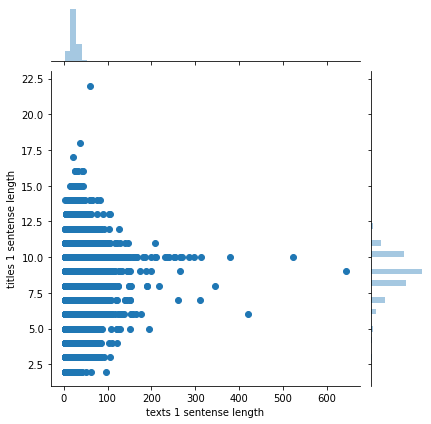
\includegraphics[width=1.0\linewidth]{sents_lens.png}
    \caption{First sentences lengths distribution}
    \label{fig:circle}
\end{figure}

\begin{figure}[H]
    \centering
    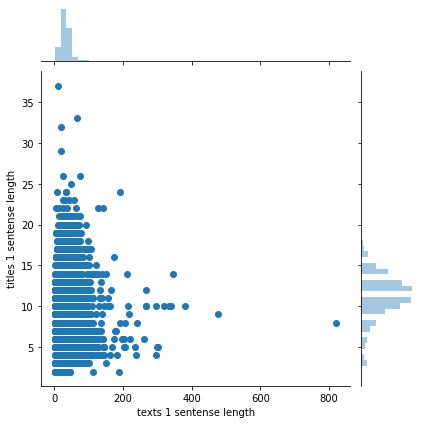
\includegraphics[width=1.0\linewidth]{lens_bpe.png}
    \caption{First sentences lengths distribution BPE}
    \label{fig:circle}
\end{figure}

\begin{figure}[H]
    \centering
    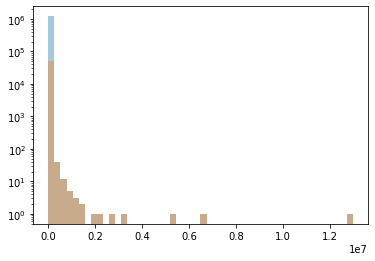
\includegraphics[width=1.0\linewidth]{vocab_not_norm_50k.png}
    \caption{Raw word count distribution at reduced vocabulary (50k words, red) over full (1.2M words, blue)}
    \label{fig:circle}
\end{figure}

\begin{figure}[H]
    \centering
    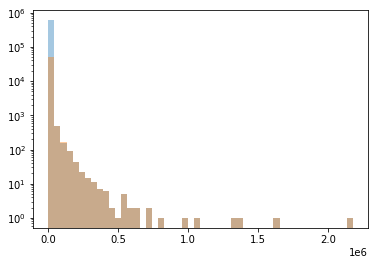
\includegraphics[width=1.0\linewidth]{voc.png}
    \caption{Lemmatized word count distribution at reduced vocabulary (50k words, red) over full (600k words, blue)}
    \label{fig:circle}
\end{figure}

\subsection{BPE}
We tried to use BPE with the youtokentome \cite{youtokentome} library. Conclusion is that for topics sharing the space with words (concept used in ABAE model) this approach doesn't seem to be much promising. Words may have several meanings, but tokens have much more and in fact have much more syntactic than semantic meanings. E.g. let's consider the attention matrix from RNN for word tokens: different words have strong relationships, but if we look at bpe matrix we rather find strong relationships between the same tokens than between different ones. But we have only qualitative analysis, for strict conclusions a quantitative analysis should be performed.
\begin{figure}[H]
    \centering
    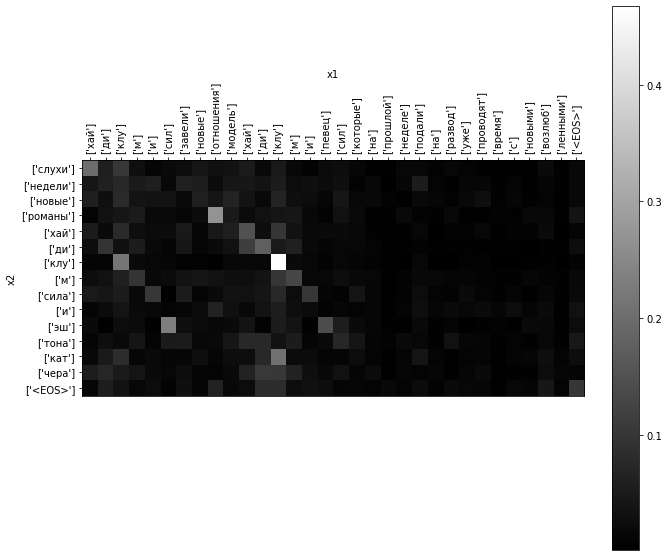
\includegraphics[width=1\linewidth]{attn_bpe.png}
    \caption{BPE attention martix}
    \label{fig:circle}
\end{figure}
\begin{figure}[H]
    \centering
    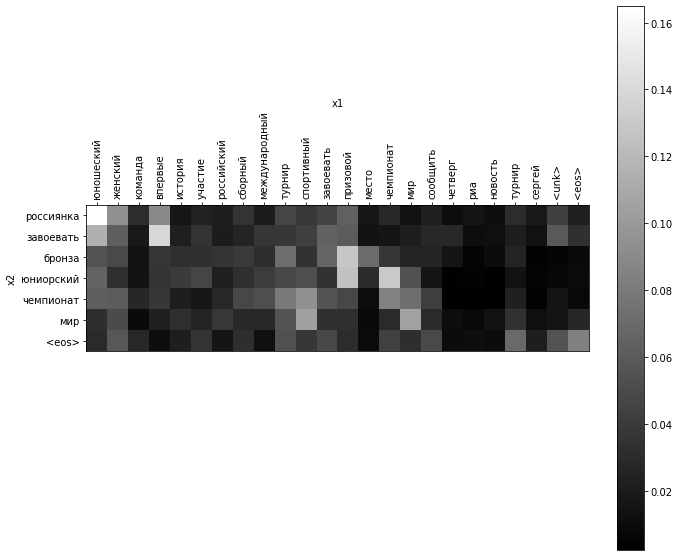
\includegraphics[width=1\linewidth]{attnnn.png}
    \caption{Words attention matrix}
    \label{fig:circle}
\end{figure}

\section{Experiments}

\subsection{Transformer + ABAE}
Training process deserves detailed description. We pretrained word vectors by gensim word2vec model with the following parameters: window size is 10, negative sampling is 5, word embedding size is 300 as in all the way down through the transformer. Vocabulary is stricted by 50000 words, other words are encountered near 1-2 times through all corpus.
ABAE aspects vectors are initiated with 100 kmeans centroids.

\subsection{RNN}
It is a seq2seq model with an attention mechanism. Principal scheme of the neural net is shown in Figure \ref{fig:rnn}.

\begin{figure}[H]
    \centering
    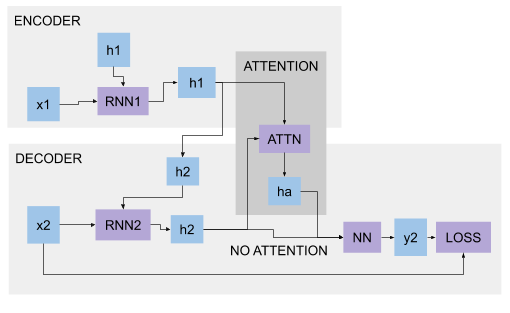
\includegraphics[width=1.0\linewidth]{rnn.png}
    \caption{Seq2Seq RNN with attention scheme. Where: RNN - Recurrent Neural Network, NN - feedforward Neural Network with one hidden layer,  x1 - input sequence, x2 - target sequence, y - prediction sequence,  h - RNN  hidden state, ATTN - attention algorithm}
    \label{fig:rnn}
\end{figure}

Parameters of the network are given in table \ref{tab:model_ps}. We used vanilla RNN cell types with a hidden size of 200. Output feedforward network NN makes conversion of sizes: 400 (200 RNN hidden + 200 RNN attention) -> 600 (NN hidden layer size) -> 50004 (embedding size).

\begin{table}[H] \label{tbl:rnn_model_parameters}
\begin{center}
\begin{tabular}[t]{|l|c|}
\hline
%\cline{2-4}
 Parameter & Value \\
\hline
Embedding dim & 300 \\
Embedding size & 50004\\
RNN cell type & RNN \\
RNN hidden size & 200 \\
NN hidden size & 600 \\
Attention & softmin euclidean distance\\
Trained parameters & 60M \\
\hline
\end{tabular}
\caption{Model parameters}
\label{tab:model_ps}
\end{center}
\end{table}


\begin{figure}[H]
    \centering
    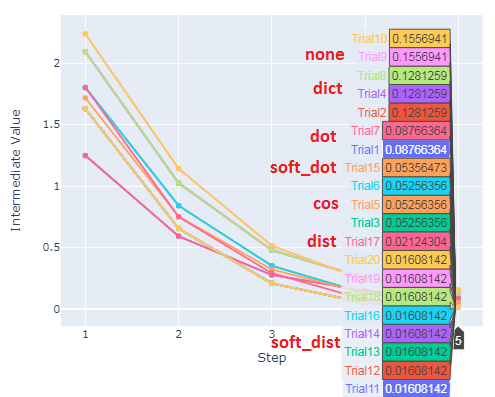
\includegraphics[width=1.0\linewidth]{attn.png}
    \caption{Attention algorithm comparison}
    \label{fig:attn}
\end{figure}

We selected euclidean distance as an attention metric after comparison with dot, softmax dot, cos, softmax cos and inverse distance (dict distance metric is experimental and isn't considered in our task). Comparison of loss function after 5 epochs with several trials on a test dataset is shown in Figure \ref{fig:attn}. Loss with softmin distance function (i.e. softmax negative distance) is 10 times lower than with no attention model and 8 times lower than cos metric.

\begin{table}[H] \label{tbl:rnn_training_parameters}
\begin{center}
\begin{tabular}[t]{|l|c|}
\hline
%\cline{2-4}
 Parameter & Value \\
\hline
optimizer  & Adam \\
learning rate & 1e-3\\
weight decay  & 1e-6 \\
batch size & 300 \\
seed & 0 \\
\hline
\end{tabular}
\caption{Train parameters}
\label{tab:statistics}
\end{center}
\end{table}

\subsection{Beam Search}
We have implemented a beam search algorithm with several options, like backward search, batch and beam reductions.

\begin{figure}[H]
    \centering
    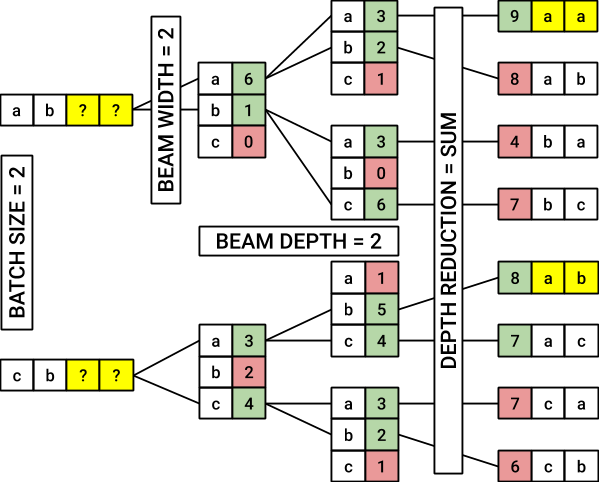
\includegraphics[width=1.0\linewidth]{beam_frw.png}
    \caption{Classic beam search with depth reduction or cumulative score}
    \label{fig:beam_fwd}
\end{figure}
Beam search implements the concept of chain of conditional probabilities between events. We use that sequence of events that have maximum likelihood over all steps. E.g. on a picture \ref{fig:beam_fwd} given two sequences ab and cb for which we want to predict next tokens. These predictions have condition (previous tokens ab and c consequently) and weights for each possible token. E.g. for sequence cb weights for the next third token are 3 for token a, 2 for b and 4 for c. If we don't use beam search (one can say use beam search with beam depth 1), we choose more probable token c and go to prediction of fourth token with sequence cbc as new condition and so on. In our example we will have weigths 3, 2 and 1 for tokens a, b and c. In this case we would choose a fourth final token and produce a resulting sequence cbca.
But what if we would choose a token on the first step? Then we would have another weights for a, b and c: 1, 5 and 4. Then we would choose b on for a fourth token and get the final sequence cbab.
If we calculate the cumulative weight of each path we will see that the last sequence has weight 8 that is more than weight 7 for the first one. We can argue about the meaning of this cumulative score or does it make sense. For probabilistic models its like a cumulative confidence about decision making. We can have small confidence on a first step but then strong on next that leads us to greater cumulative confidence.
Beam search allows us to consider more paths. We can change beam width and depth. In a fact we can calculate all possible variants, there are N**D, where N - number of all possible tokens, D - number of predicting tokens. It is an exponential time task and requires a huge computational resources. In place of width we can stop beam if it achieves special termination  token e.g. <eos>, but we can't know (for non exponential time) does it achieve it or doesn’t. And put some restrictions on length or time for algorithm.

\begin{figure}[H]
    \centering
    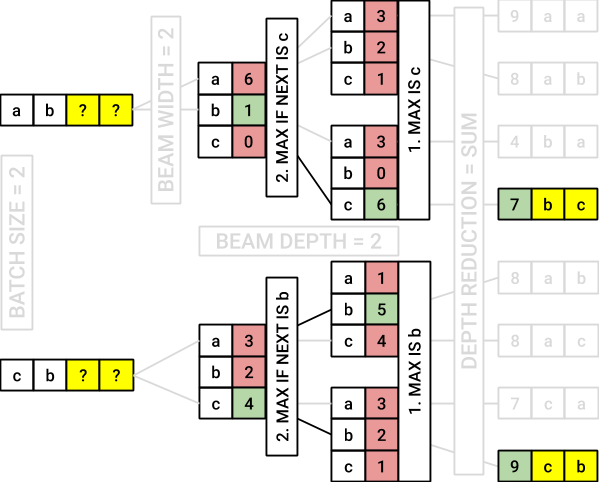
\includegraphics[width=1.0\linewidth]{beam_bkw.png}
    \caption{Backward algorithm}
    \label{fig:beam_bkw}
\end{figure}

There is another variant how to calculate cumulative weight or rather choose right sequence. After calculating weights we can choose maximum weight token on a lst step and then go to previous step only in tokens that could produced max token. E.g. on picture \ref{fig:beam_bkw} maximum token is b with weight 5. On previous step b can be achieved from a and c token. We choose c with weight 5 though it doesn't lead to b directly. 

\begin{figure}[H]
    \centering
    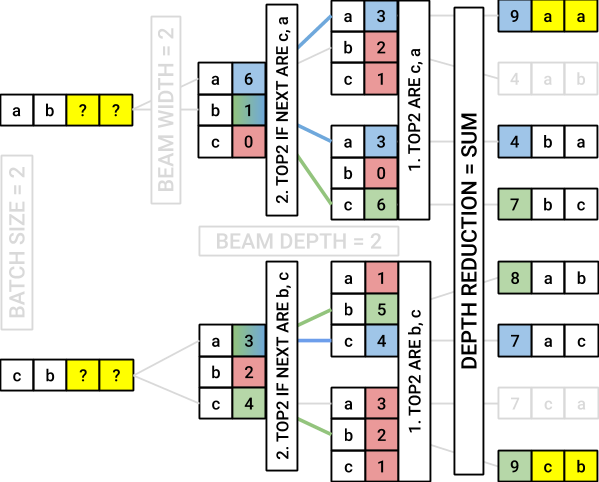
\includegraphics[width=1.0\linewidth]{beam_bkw_topk.png}
    \caption{Backward algorithm (topk)}
    \label{fig:beam}
\end{figure}

We can choose top k tokens at last prediction and propagate the algorithm independently.

\begin{figure}[H]
    \centering
    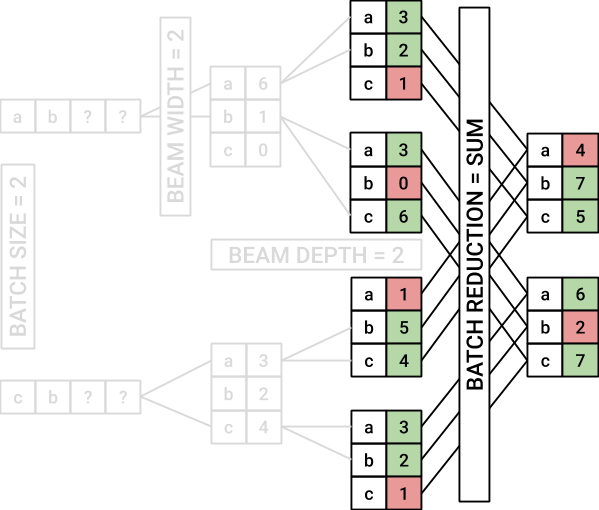
\includegraphics[width=1.0\linewidth]{beam_batch_red.png}
    \caption{Batch reduction for many to one sequence generation}
    \label{fig:beam}
\end{figure}
For topic generation where we have several sequences at text and one at topic we could try to do batch reductions to achieve cumulative batch likelihood for a token.

\begin{figure}[H]
    \centering
    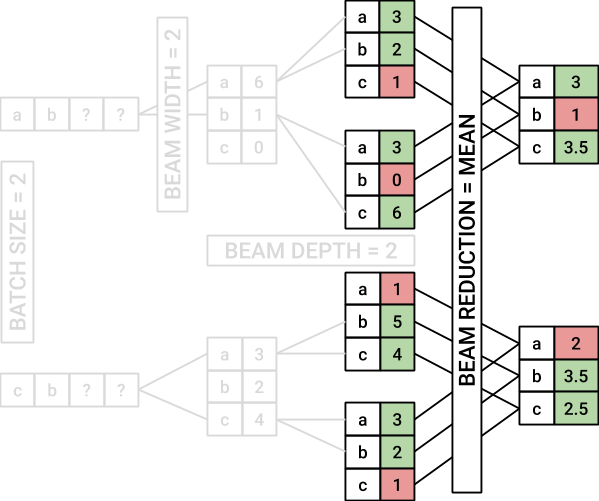
\includegraphics[width=1.0\linewidth]{beam_beam_red.png}
    \caption{Beam reduction to share information between beams}
    \label{fig:beam}
\end{figure}

If we have several beams we can make a beam reduction to achieve cumulative beams likelihoods for next propagation. 

\begin{figure}[H]
    \centering
    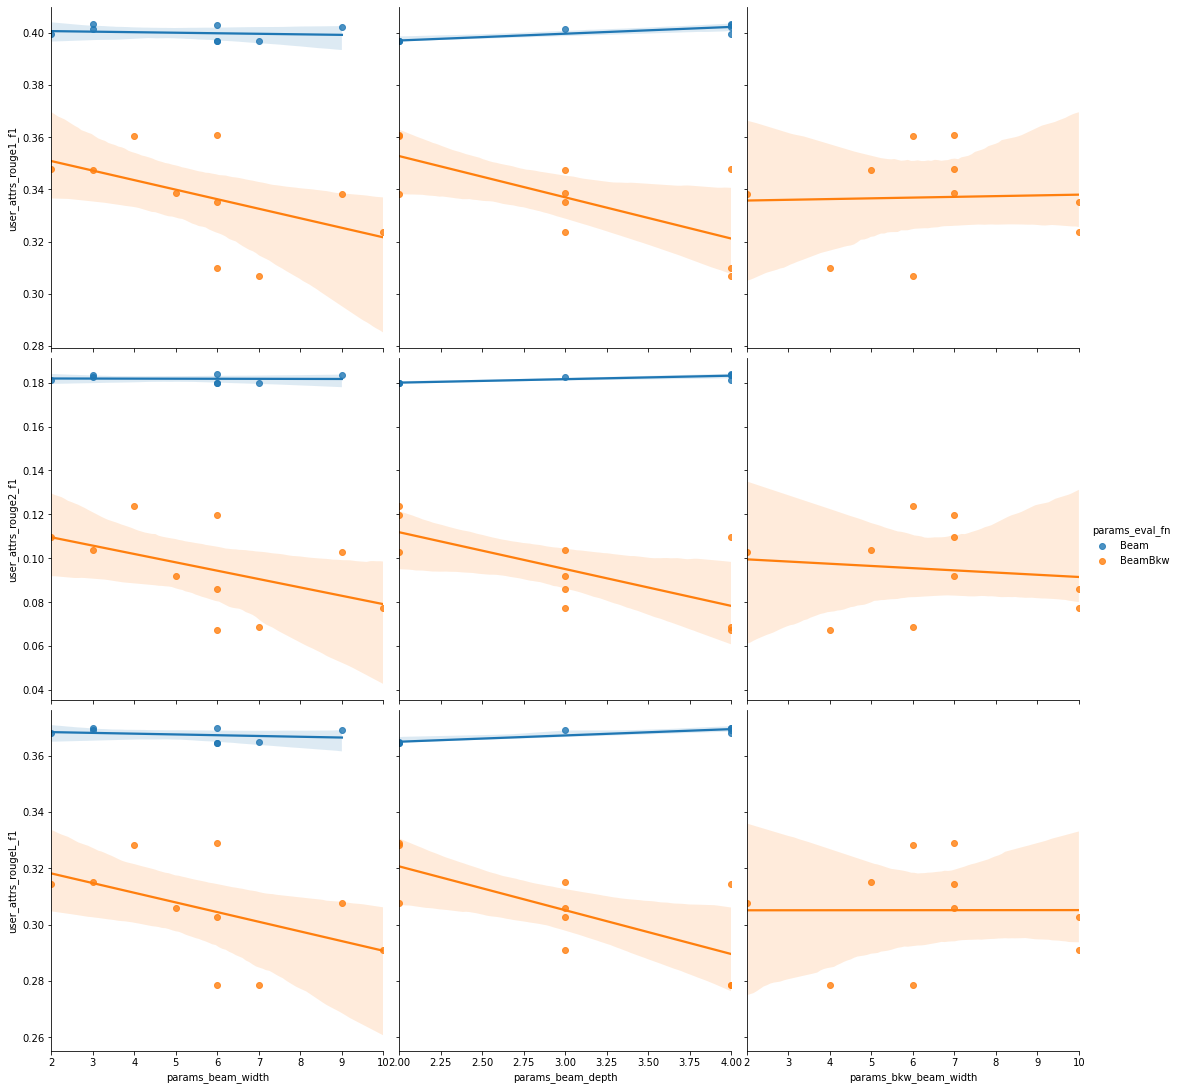
\includegraphics[width=1.0\linewidth]{beam.png}
    \caption{First sentences lengths distribution}
    \label{fig:beam}
\end{figure}

From the comparison (Picture \ref{fig:beam}) we can conclude that forward-backward beam search has worse prediction than simple forward beam search. Also we see a small positive relationship between scores and beam depth and no relationship between beam width. Comparison made on 1000 samples from test dataset.


\subsection{Metrics}
We used ROUGE metrics to evaluate summarization quality. Also we measured length ratio and non ordered words coincidence (set).

\subsection{Experiment Setup}

Dataset was splitted into 3 parts: train, loss and validation with 70\%, 20\% and 10\% of samples. We used only the first sentence for training, because that reduces training time and there is a hypothesis that the topic of the news consists mostly of words of the first sentence. We used a GPU Tesla P100-PCIE-16GB.


\subsection{Baselines}
We got baseline results from papers \cite{gavrilov2018self} and \cite{gusev2019importance}.

\section{Results}

Scores comparison is given in the table \ref{tab:scores}. Scores obtained on 100k samples of the test dataset as mean of individual pairs scores. Outputs are given in the table \ref{tab:output}.

\begin{table}[tbh!]
\begin{center}
\setlength{\tabcolsep}{2pt}
\begin{tabular}[t]{|l|c|c|c|ccccccc|}
\hline
model & tok & oov & input & R-1-f & R-1-r & R-2-f & R-2-r & R-L-f & R-L-r & R-m-f  \\
\hline
T+A (greedy) & raw & 7\% & 1S & 12.66 & 12.60 & 2.10 & 2.11 & 12.25 & 12.21 & 9.00\\
RNN (greedy) & bpe & 0\% & 1S & 29.90 & 29.71 & 15.21 & 15.15 & 28.22 & 28.04 & 24.44 \\
T (greedy) & lem & 2\% & 1S & 37.56 & 32.40 & 10.05 & 8.50 & 31.55 & 27.10 & 26.39 \\
RNN (greedy) & raw & 7\% & 1S & 34.67 & 34.66 & 15.65 & 15.70 & 32.38 & 32.38 & 27.57 \\
RNN (greedy) & lem & 2\% & 1S & 38.42 & 37.82 & 16.62 & 16.41 & 35.67 & 35.12 & 30.24 \\
T+A (greedy) & lem & 2\% & 1S & 41.17 & 40.47 & 15.40 & 15.15 &
36.80 & 36.19 & 31.12 \\
RNN (beam 10-10-3) & lem  & 2\% &  1S & 39.60 & 39.14 & 17.97 & 17.78 & 36.84 & 36.42 & 31.47 \\
RNN (beam 2-2-8) & lem  & 2\% &  1S & 40.19 & 40.39 & 18.29 & 18.37 & 37.37 & 37.57 & 31.95\\
RNN (beam 10-2-10) & lem & 2\% & 1S & 40.17 & 40.58 & 18.49 & 18.66 & 37.34 & 37.72 & 32.00 \\
\hline
First Sentence \cite{gavrilov2018self} & bpe & 0\% & 1S & 24.08 & 45.58 & 10.57 & 21.30 & 16.70 & 41.67 & 17.12 \\
seq2seq-words-25m \cite{gusev2019importance} & raw & ?\% & 400T & 36.96 & 35.19 & 19.68 & 19.02 & 34.30 & 33.60 & 30.31 \\
UT w/ smoothing \cite{gavrilov2018self} & bpe & 0\% & 3kT &  39.31 & 37.10 & 21.82 & 20.66 & 36.32 & 35.37 & 32.48 \\
Encoder-Decoder \cite{gavrilov2018self} & bpe & 0\% & 1S & 39.10 & 38.31 & 22.13 & 21.75 & 36.34 & 36.34 & 32.52 \\
UT \cite{gavrilov2018self}   & bpe & 0\% & 3kT & 39.75 & 37.62 & 22.15 & 21.04 & 36.81 & 35.91 & 32.90 \\
seq2seq-bpe-25m \cite{gusev2019importance} & bpe & 0\% & 800T & 40.30 & 38.83 & 22.94 & 22.18 & 37.50 & 37.01 & 33.58 \\
copynet-bpe-43m \cite{gusev2019importance} & bpe & 0\% & 800T & 41.61 & 40.33 & 24.46 & 23.76 & 38.85 & 38.51 & 34.97 \\
\hline
\end{tabular}
\caption{Rouge1-2-L-mean recall and f1 scores ordered by Rouge mean f1 score on RIA dataset. There tok - tokenization type, input - length of the input (S - sentence, T - token), oov - out of vocabulary words (from total words count), T - transformer, A - ABAE, UT - Universal Transformer. Beam [first token beam width]-[other tokens beam width]-[max beam depth].}
\label{tab:scores}
\end{center}
\end{table}

Our models have worse score compared with related works. Also we got very low scores for Transformer with raw text normalization (Why?). Beam search raises scores on 1-2 points. We noticed that depth of the beam is more important than its width. We do not provide beam search results for Transformer because we didn't calculate them enough (100k samples). But on 1k samples it also gives  1-2 points to scores.

\begin{table}[H]
\begin{center}
\begin{tabular}[c]{|p{1cm}|p{11cm}|}
\hline
\multicolumn{2}{|c|}{\text{raw 1}} \\
\hline
input & россия <unk> от арабского мира и международного сообщества не желая участвовать во встрече министров иностранных дел по сирии в париже заявил в четверг глава мид франции ален жюппе \\
target & россия <unk> не приехала на встречу по сирии мид франции \\
output & мид франции россия <unk> от арабского мира заявил ален жюппе \\
\hline
\multicolumn{2}{|c|}{\text{raw 2}} \\
\hline
input & действия россии которая ввела эмбарго на импорт продовольственных товаров из ес сша и других западных стран принявших ранее санкции в отношении нее не стали сюрпризом их вероятность следовало просчитать озвучила в четверг комментарий президента латвии <unk> <unk> его лига <unk> \\
target & руководители латвии советуют производителям искать другие рынки сбыта \\
output & <unk> <unk> <unk> <unk> <unk> <unk>\\
\hline
\multicolumn{2}{|c|}{\text{lem 1}} \\
\hline
input & консульский отдел американский посольство москва вторник днём перестать принимать посетитель ремонт сообщаться сайт посольство \\
target & консульский отдел посольство сша москва принимать посетитель\\
output & отдел посольство сша москва перестать принимать посетитель\\
\hline
\multicolumn{2}{|c|}{\text{lem 2}} \\
\hline
input & читатель иностранный издание вступить дискуссия насколько закрытие проект южный поток расширение мощность трубопровод голуба поток повлиять благополучие страна евросоюз также дальнейший быть развиваться отношение россия турция\\
target & зарубежный пользователь отказ рф южный поток блестящий ход\\
output & читатель сми мочь южный проект поток снизить\\
\hline
\multicolumn{2}{|c|}{\text{bpe 1}} \\
\hline
input & жители украины жалуются в координационный штаб общественной палаты россии на массовые нарушения своих прав заявил риа новости во вторник представитель оп\\
target & украинцы жалуются в общественную палату рф на массовые нарушения прав\\
output & жители украины жалуются на массовые нарушения прав человека\\
\hline
\multicolumn{2}{|c|}{\text{bpe 2}} \\
\hline
input & лабораторное исследование выявило у четырех больных госпитализированных из кировского санатория колос с симптомами острой кишечной инфекции возбудитель сальмонеллеза сообщила в пятницу риа новости начальник отдела эпиднадзора управления роспотребнадзора по кировской области любовь опарина\\
target & отдыхающие санатория под кировом заболели сальмонеллезом\\
output & медики компенсацию поставили в санатории самарской области нехватки школьников\\
\hline
\end{tabular}
\caption{Output samples}
\label{tab:output}
\end{center}
\end{table}

\pagebreak

\section{Conclusions}
We used 2 methods for text summarization (RNN and Transformers), ABAE model for topic generation, Transformer + ABAE model for topic generation and summarization and several text normalizations algorithms. 
Conclusions and inferences:
\begin{enumerate}
\item We intended to implement Transformer + ABAE for text summarization and we've done it.
\item Transformer + ABAE model raised scores by several points in comparsion with simple Transformer.
\item Unfortunately we didn't try to change summarization topic by ABAE vectors due lack of time. In short: we need another dataset with tagged topics for this task.
\item We did several text preprocessing pipelines that led us to conclusion that BPE encoding is a very promising approach, that doesn't reduce dataset vocabulary, though it got worse scores on our models.
\item We implemented beam search with different options. We noticed that depth of beam search is more important than width though it leads to 
\item We implemented simple seq2seq model with attention to compare it with transformer, and noticed that there is not much difference in scores between them.
\item Our scores is lower than scores in related works \cite{gavrilov2018self} \cite{gusev2019importance}. There is several reasons from our point of view: our main task is to implement Transformer and ABAE model not to raise score of text summarization (but it's of course implied), we used self-made models and we did small hyper-parameters tuning because of lack of time.
\item By analysing attentions matrices of RNN model we noticed that attention with BPE tokens seems more syntactic than semantic as one's with word tokens.
\item We implemented several beams reductions (like batch reduction or beam reduction) for beam search but didn't try them and will do so in future works.
\item Project turned out to be mostly research or even educational but this experience will be useful in our future projects.
\end{enumerate}

\pagebreak

\bibliographystyle{unsrt}
\bibliography{lit}


\end{document}